%!TEX program = xelatex

\documentclass[twocolumn]{report}

\usepackage[
  paper=letterpaper,
  nofoot,nomarginpar,nohead,
  margin=1cm,
  tmargin=1.2cm
]{geometry}

%%%%%%%%%%%%%%%%%%%%%%%%%%%%%%%%%%%%%%%%%%%%%%%%%%%%%%%%%%%%%%%%%%%%%%%%%%%%%%%%

\makeatletter
\newcommand\notsotiny{\@setfontsize\notsotiny{6.5}{8}}
\makeatother
\pagestyle{empty}

%%%%%%%%%%%%%%%%%%%%%%%%%%%%%%%%%%%%%%%%%%%%%%%%%%%%%%%%%%%%%%%%%%%%%%%%%%%%%%%%

\usepackage{unicode-math}
\setmainfont[
	BoldFont = texgyreschola-bold.otf,
	BoldItalicFont = texgyreschola-bolditalic.otf,
	ItalicFont = texgyreschola-italic.otf
]{texgyreschola-regular.otf}
\setmathfont{texgyreschola-math.otf}

%%%%%%%%%%%%%%%%%%%%%%%%%%%%%%%%%%%%%%%%%%%%%%%%%%%%%%%%%%%%%%%%%%%%%%%%%%%%%%%%

\usepackage{tikz}

%%%%%%%%%%%%%%%%%%%%%%%%%%%%%%%%%%%%%%%%%%%%%%%%%%%%%%%%%%%%%%%%%%%%%%%%%%%%%%%%

\usepackage{tabularx}

\newcolumntype{P}{X}%
\newcolumntype{L}{>{\raggedright\arraybackslash}X}%
\newcolumntype{R}{>{\raggedleft\arraybackslash}X}%
\newcolumntype{C}{>{\centering\arraybackslash}X}%
\newcolumntype{q}[1]{>{\centering\arraybackslash\hspace{0pt}}p{#1}}

\usepackage{multirow}

%%%%%%%%%%%%%%%%%%%%%%%%%%%%%%%%%%%%%%%%%%%%%%%%%%%%%%%%%%%%%%%%%%%%%%%%%%%%%%%%

\newcommand{\drawwings}[1]{
  \draw [very thick] (-1,#1) -- (+1,#1);
}
\newcommand{\drawlowwings}{\drawwings{-0.09}}
\newcommand{\drawmidwings}{\drawwings{+0.00}}
\newcommand{\drawhighwings}{\drawwings{+0.09}}

\newcommand{\drawtail}[3]{
  \draw [very thick] (0,0) -- (0,#2);
  \draw [very thick] (-#3,#1) -- (+#3,#1);
}
\newcommand{\drawlowtail}[2][0.35]{\drawtail{-0.05}{#2}{#2}}
\newcommand{\drawmidtail}[2][0.35]{\drawtail{+0.00}{#2}{#2}}
\newcommand{\drawhightail}[2][0.35]{\drawtail{+0.05}{#2}{#2}}


\newcommand{\drawttail}[2][0.3]{
  \draw [very thick] (0,0) -- (0,#1);
  \draw [very thick] (-#2,#1) -- (+#2,#1);
}

\newcommand{\drawfuselage}[1][0.15]{
  \draw [very thick] (0,0) [fill=white] circle (#1);
}

\newcommand{\drawengines}[3][0.1]{
  \draw [very thick] (+#3,#2) [fill=white] circle (#1);
  \draw [very thick] (-#3,#2) [fill=white] circle (#1);
}
\newcommand{\drawverylowengines}[2][0.1]{\drawengines[#1]{-0.15}{#2}}
\newcommand{\drawlowengines}[2][0.1]{\drawengines[#1]{-0.09}{#2}}
\newcommand{\drawmidengines}[2][0.1]{\drawengines[#1]{+0.00}{#2}}
\newcommand{\drawhighengines}[2][0.1]{\drawengines[#1]{+0.05}{#2}}

\newcommand{\drawstation}[3][-0.3]{
  \draw (#2,#1) -- ++(0,-0.2) node [anchor=north] {\footnotesize #3};
}

\newcommand{\drawstations}[3][0.0]{
  \draw (#2,-0.3) -- ++(#1+0.08,-0.2);
  \draw (#2,-0.3) -- ++(#1-0.08,-0.2);
  \draw (#2,-0.3) ++(#1,-0.2) node [anchor=north] {\footnotesize #3};
}


%%%%%%%%%%%%%%%%%%%%%%%%%%%%%%%%%%%%%%%%%%%%%%%%%%%%%%%%%%%%%%%%%%%%%%%%%%%%%%%%

\begin{document}

F4U
\par\medskip
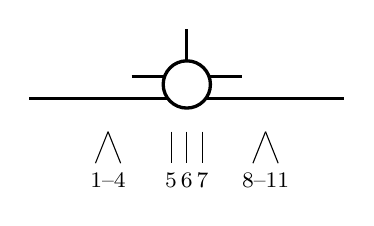
\begin{tikzpicture}[scale=2]
\drawlowwings
\drawhightail{0.35}
\drawfuselage
\drawstations{-0.5}{1--4}
\drawstation{-0.1}{5}
\drawstation{+0.0}{6}
\drawstation{+0.1}{7}
\drawstations{+0.5}{8--11}
\end{tikzpicture}
\bigskip

B-26B/C
\par\medskip
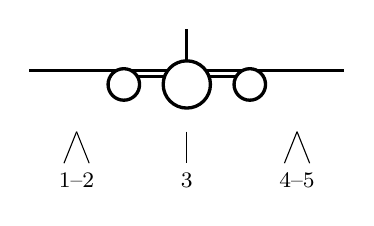
\begin{tikzpicture}[scale=2]
\drawhighwings
\drawhightail{0.35}
\drawfuselage
\drawmidengines{0.4}
\drawstations{-0.7}{1--2}
\drawstation{+0.0}{3}
\drawstations{+0.7}{4--5}
\end{tikzpicture}
\par\medskip
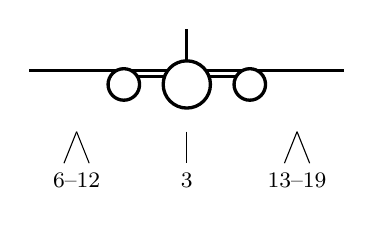
\begin{tikzpicture}[scale=2]
\drawhighwings
\drawhightail{0.35}
\drawfuselage
\drawmidengines{0.4}
\drawstations{-0.7}{6--12}
\drawstation{+0.0}{3}
\drawstations{+0.7}{13--19}
\end{tikzpicture}
\bigskip


B-26K
\par\medskip
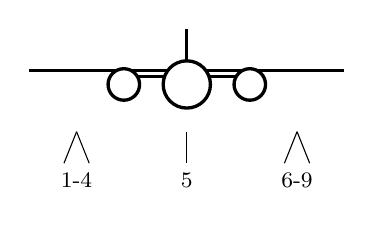
\begin{tikzpicture}[scale=2]
\drawhighwings
\drawhightail{0.35}
\drawfuselage
\drawmidengines{0.4}
\drawstations{-0.7}{1-4}
\drawstation{+0.0}{5}
\drawstations{+0.7}{6-9}
\end{tikzpicture}
\bigskip

B-29A
\par\medskip
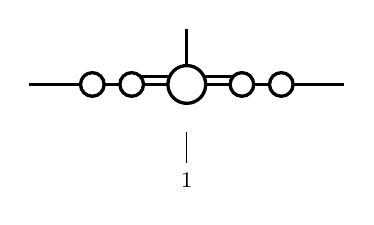
\begin{tikzpicture}[scale=2]
\drawmidwings
\drawhightail{0.35}
\drawfuselage[0.12]
\drawmidengines[0.075]{0.35}
\drawmidengines[0.075]{0.60}
\drawstation{+0.0}{1}
\end{tikzpicture}
\bigskip


F-80C
\par\medskip
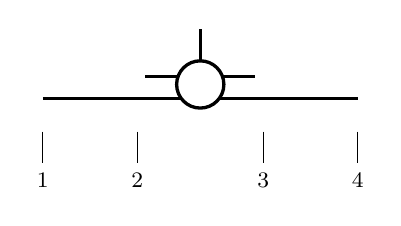
\begin{tikzpicture}[scale=2]
\drawlowwings
\drawhightail{0.35}
\drawfuselage
\drawstation{-1.0}{1}
\drawstation{-0.4}{2}
\drawstation{+0.4}{3}
\drawstation{+1.0}{4}
\end{tikzpicture}
\par\medskip
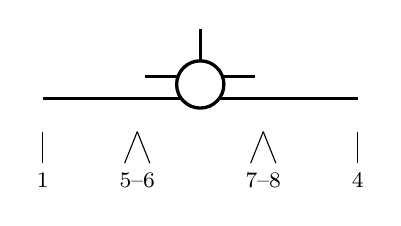
\begin{tikzpicture}[scale=2]
\drawlowwings
\drawhightail{0.35}
\drawfuselage
\drawstation{-1.0}{1}
\drawstations{-0.4}{5--6}
\drawstations{+0.4}{7--8}
\drawstation{+1.0}{4}
\end{tikzpicture}
\bigskip

AD-4
\par\medskip
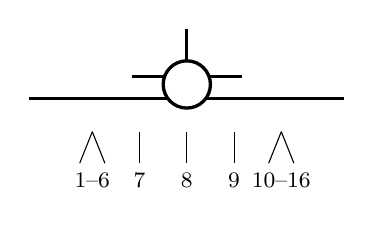
\begin{tikzpicture}[scale=2]
\drawlowwings
\drawhightail{0.35}
\drawfuselage
\drawstations{-0.6}{1--6}
\drawstation{-0.3}{7}
\drawstation{+0.0}{8}
\drawstation{+0.3}{9}
\drawstations{+0.6}{10--16}
\end{tikzpicture}
\bigskip

F-4C
\par\medskip
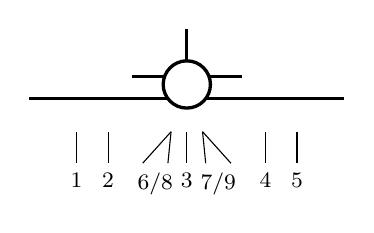
\begin{tikzpicture}[scale=2]
\drawlowwings
\drawhightail{0.35}
\drawfuselage
\drawstation{-0.7}{1}
\drawstation{-0.5}{2}
\drawstation{+0.0}{3}
\drawstation{+0.5}{4}
\drawstation{+0.7}{5}
\drawstations[-0.1]{-0.1}{6/8}
\drawstations[+0.1]{+0.1}{7/9}
\end{tikzpicture}
\bigskip

Meteor
\par\medskip
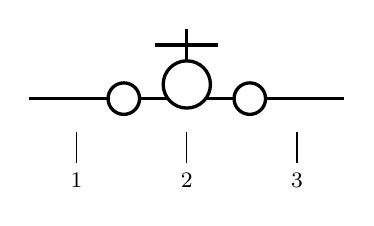
\begin{tikzpicture}[scale=2]
\drawlowwings
\drawtail{0.25}{0.35}{0.2}
\drawfuselage
\drawlowengines{0.4}
\drawstation{-0.7}{1}
\drawstation{+0.0}{2}
\drawstation{+0.7}{3}
\end{tikzpicture}
\par\medskip
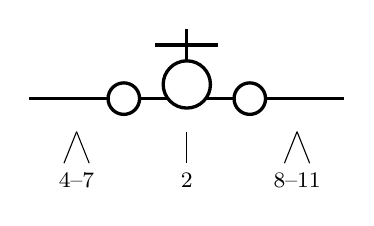
\begin{tikzpicture}[scale=2]
\drawlowwings
\drawtail{0.25}{0.35}{0.2}
\drawfuselage
\drawlowengines{0.4}
\drawstations{-0.7}{4--7}
\drawstation{+0.0}{2}
\drawstations{+0.7}{8--11}
\end{tikzpicture}
\bigskip

Sea Fury
\par\medskip
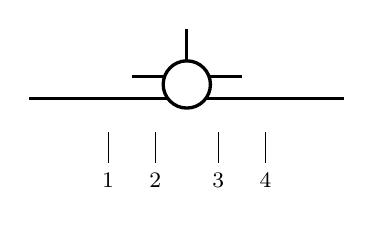
\begin{tikzpicture}[scale=2]
\drawlowwings
\drawhightail{0.35}
\drawfuselage
\drawstation{-0.5}{1}
\drawstation{-0.2}{2}
\drawstation{+0.2}{3}
\drawstation{+0.5}{4}
\end{tikzpicture}
\par\medskip
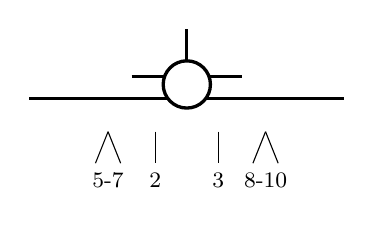
\begin{tikzpicture}[scale=2]
\drawlowwings
\drawhightail{0.35}
\drawfuselage
\drawstations{-0.5}{5-7}
\drawstation{-0.2}{2}
\drawstation{+0.2}{3}
\drawstations{+0.5}{8-10}
\end{tikzpicture}
\bigskip

Yak-9D
\par\medskip
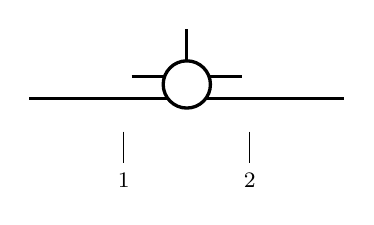
\begin{tikzpicture}[scale=2]
\drawlowwings
\drawhightail{0.35}
\drawfuselage
\drawstation{-0.4}{1}
\drawstation{+0.4}{2}
\end{tikzpicture}
\bigskip

Il-10
\par\medskip
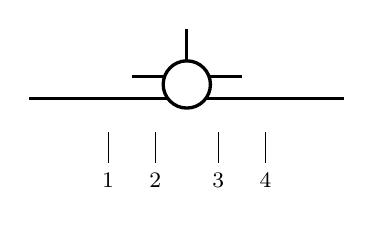
\begin{tikzpicture}[scale=2]
\drawlowwings
\drawhightail{0.35}
\drawfuselage
\drawstation{-0.5}{1}
\drawstation{-0.2}{2}
\drawstation{+0.2}{3}
\drawstation{+0.5}{4}
\end{tikzpicture}
\bigskip



\end{document}
